\documentclass{standalone}

\usepackage{circuitikz}

\begin{document}

% INT_AY20_MP3_L27_Fig01_Mag_flux_through_circle.png

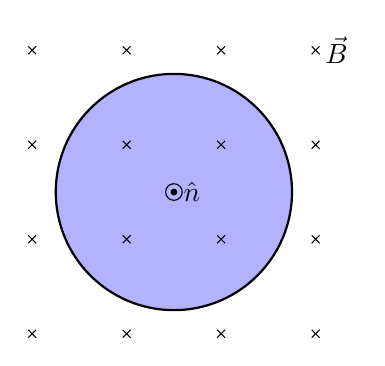
\begin{tikzpicture}

	% Circle with thick boundary
	
	\filldraw [thick, draw = black, fill = blue!30] (0, 0) circle (1.5 cm);
	
	% Normal vector
	
	\filldraw (0, 0) circle (1 pt);
	\draw (0, 0) circle (3 pt) node [right] {${\hat n}$};
	
	% Magnetic field
	
	\foreach \x in {-1.8, -0.6, 0.6, 1.8}
	\foreach \y in {-1.8, -0.6, 0.6, 1.8}
	{
		\draw (\x + 0.05, \y + 0.05) -- (\x - 0.05, \y - 0.05);
		\draw (\x + 0.05, \y - 0.05) -- (\x - 0.05, \y + 0.05);
	}
	
	\node [right] at (1.8, 1.8) {${\vec B}$};

\end{tikzpicture}

\end{document}